
\documentclass[a4paper,12pt,oneside]{article}

\usepackage[english]{babel}
\usepackage[utf8]{inputenc}
\usepackage[T1]{fontenc}
\usepackage{listings}
\usepackage{amsmath}
\usepackage{amsthm}
\usepackage{url}
\usepackage{verbatim}
\usepackage{graphicx}

\newtheorem{theorem}{Theorem}
\newtheorem{lemma}[theorem]{Lemma}

\title{Advanced Algorithms - Euclidean Travelling Salesman Problem}
\author{Samuel Wej\'eus \\ \lowercase{wejeus@kth.se} \and Peter Boström \\ \lowercase{pbos@kth.se} }

\begin{document}
\maketitle

\section{Introduction}
In the fields of computer science and mathematical optimization a well known problem is the \textit{tradelling salesman problem, or TSP}. The problem is often stated as follows: \textit{given a list of cities and their pairwise distances, find the shortest possible path that visit each city exactly once and then return to the start position}. It is easy to see how this can be transformed into a mathematical representation by using a graph. Each city is a node, let there be an edge from each city to every other city, each representing the distance between the two. The solution to the problem must then be an ordered subset of the edges with the constraints that two edges immediately following each other must end in a common vertex and there must be exactly $n$ vertices each occurring exactly once.

It is well know that the TSP is NP-complete and we will not dwell on details only mention that no deterministic algorithm \footnote{Deterministic used in the sense of reduction based problem structure, i.e. no guarantee in correctness of subproblems.} that finds an optimal solution currently exists, instead the most commonly used approach is to find some (possible bad) solution and then successively improve this solution until some halting criteria is met.

This report only touches the Euclidean TSP, some methods proposed may not be usable, on general-case TSP.

\section{Held-Karp Lower bound}

As finding optimal results is very hard (so long as NP isn't within P), we can't expect to find optimal results within polynomial time. In order to measure how good an algorithm is, we can use a lower bound for a TSP tour which can be found in polynomial time. This is done using the Held-Karp lower bound, which is the solution to the linear programming relaxation of the TSP, which can actually be computed in polynomial time\cite{bound}. This bound seems to average about 0.8\% below the optimal tour length, but is only guaranteed to be within 2/3 of the optimal tour. 

Also, it's not feasible to construct this lower bound exactly for very large tours, for which an iterative version, which keeps close to the HK bound, has been proposed instead. Both versions of these methods however were however of very great use to us, as we'd measure our algorithms directly on Kattis' data. It's noteworthy however, because it provides some kind of measure, and can in some way say how far a solution could possibly be from the optimal one.

\section{Tour construction}

As the given problem is NP-hard, computing an exact solution for the tour isn't really to hope for. Exact solutions for the travelling-salesman problem can be found with dynamic programming in $O(2^n)$ time with inclusion-exclusion\cite{exact}.

This isn't usable for us, as we need to construct tours within polynomial time. Our approach will be to construct a tour ``quickly'' and attempt local optimizations. There are a few different we could use:

\subsection{Random tour}

Creating a random tour consists of simply shuffling the cities, which is $O(n)$, for us it wasn't very beneficial, and the locally-optimized degenerates from this algorithm were never as good as nearest-neighbour for instance. 

\subsection{Nearest Neighbour}

Perhaps the easiest non-naive tour construction algorithm, nearest neighbour starts in any city, and goes to the closest previously-unvisited city. After all cities are visited, the tour ends by going back to where we came from. This is the initial-tour algorithm we went with, it gave the best results after local optimizations.

From each city, checking distance to all neighbours is $O(n)$, as there are $n$ cities considered, our total time will be $O(n^2)$.

\subsection{Greedy}

Similar to Kruskal's MST algorithm, we try to include the smallest edge possible into our tour. No two edges may ever end in the same city, nor can any city have two outgoing edges. We must also avoid creating a cycle with less than $n$ edges, that is, only the final edge may close the tour.

We sort the edges, and always select the shortest one, discarding ones which would violate above criterion. In order to avoid creating a cycle in the above construction, we use an union-find structure, to assert that the edges join two disjoint sets.

Experimentally, we found the greedy algorithm to work better than nearest neighbour in some cases, and worse in other. We heard that this algorithm was supposed to perform better than nearest-neighbour, but when uploading to Kattis, our testing framework, this algorithm actually gave a worse result. This may be in conjunction with how we perform our local optimizations etc. This initial tour seems to make our algorithm stuck in a worse local maxima.

Also, in our case, it seemed more beneficial to spend the extra computing time on more repeated iterations on a nearest-neighbour solution, than to compute a greedy solution first. This may be due to a flaw in our implementation, as others report a better progress with it.

\subsection{Other tour construction algorithms}

Several other tour-construction algorithms exist, but were not attempted by us, due to a lack of time. They're good to mention though, future work could consider them as candidates for starting points.

Insertion heuristics start by a subtour and insert other cities into them. Nearest-insertion works by choosing the shortest edge, and making a subtour of it, then insert the cities closest to one of the cities in the tour, and insert it. Repeat until finished. Convex-hull works by finding the convex hull of all the cities, and inserting all other cities into it iteratively, as cheap as possible.

Variants of Christofides' algorithms works by forming minimal spanning trees from the cities. They guarantee a good worst-case ratio, and might be quick enough to use.

We don't know how these tour-construction algorithms are affected by the local-optimization algorithms, they could provide both a better, or worse, local maxima, depending on methods used.

\section{Local optimization}

After arguing how to find the best possible starting tour we now look at how this tour can be improved further. Methods used typically builds on techniques to reconstruct the tour by making path changes. The more popular methods is \textit{2OPT, 3OPT} and \textit{Lin-Kernighan}. Starting with the foremost, in 2OPT we try to find a better tour by successively testing if an exchange of two edges at a time would result in an improvement of tour cost, if so perform the exchange and continue with an other two pair of nodes.

Regarding 3OPT and Lin-Kernighan, or LK for short, both can be seen as extensions of 2OPT - building on the same idea of edge exchange where in 3OPT you test three edges at a time and LK can be seen as a generalization to $k$ edges but the actual edges exchanged varies at each iteration. The running time for a 3OPT step is usually $O(n^3)$, unfeasible to run totally given our time restriction. Lin and Kernighan's variable $k$-opt algorithm is approximately $O(n^{2.2})$, and outperforms 3OPT easily\cite{lk}. In fact, LK seems to produce optimal results with impressively high frequency, though only being an approximation algorithm.

To speed up these steps, one can choose to only consider $k$ neighbours from each city, and restrict the search. Using this heuristic with $k=20$ we were able to cut running times some, without messing up the end results. Considering $k$ neighbours from each city gives 2OPT a run-time of $O(n*k)$, but results are no longer 2-optimal.

The variation in how many edges are exchanged at one time gives the various techniques different characteristics, namely difference in running time and cost of total tour found. The difference in tour cost is obviously expected since they are all \textit{local} optimization techniques and no guarantee exists that any local improvement actually is a part of any global \textit{optimal} solution (side note: this is what we refer to by \textit{non-deterministic} in the introduction, see footnote 1).

All three local optimization procedures given above have different aspects and properties that make the unique. From results given in \cite{localopt} we see that a higher running, on average, normally produces a better tour cost. As an example taken from \cite{localopt}, the difference in running time between LK and 2OPT on an input size of $10^6$ is 2650(LK) vs 940(2OPT) seconds and the average excess over Held-Karp lower bound is 2.0 vs 4.9 in favor of LK. But if running time is of more importance the higher tour cost might be acceptable. This shows that there is no clear definition of \textit{"best"} approach for local optimization instead its up to the needs of the context. 

In our case, we had a time restriction that prevented us from running 3OPT, completely at least. Aside from 2OPT we ran an extension to it known as 2.5OPT, and each time new edges were swapped in, we attempted to insert another city in between them. This doesn't destroy time complexity, as the 2OPT step generating the 2 edges being swapped is far more expensive than these linear searches. 2.5OPT was fruitful and with it we managed to score a few more points relatively easy. In a final step, because this \emph{half-opt} technique is cheap enough, we iterated through all final edges, and attempted a to insert any city in between them, which was also fruitful. In fact, it also got the tour out of a local maximum, and we could perform 2OPT some more, with small, but not non-existent, effect.

\subsection{Local maxima/minima}
When performing a local optimization we need to start the procedure at some point. The choice of start point can pose an impact on the quality of the total tour. This is due to the fact that, depending on start point, it is possible for the algorithm used to hit different local maxima/minima in varied order which in turn can affect other local maxima/minima given various results.

When referring to local maxima/minima we of course refer to the possible choice of exchanging edges. As an example a decision to exchange edge pair $x$ at time $T_0$ giving an intermediate result of $S$, now since our decision at $T_0$ we continue to $T_1$ \textit{with a reduced set of possible next action} due to the decision at $T_0$, if instead we would start at $T_1$ we would have a greater set of possible actions and, perhaps, one of those would give a result $\hat{S} > S$.

A good start node would be one that avoids removing a local maxima/minima that would be a part of the optimal solution as a response of encountering some other maxima/minima. We were unable to find any theory to build or choice of "good" start node on and are highly doubtful that such a choice is possible due to the fact of NP-completeness of the TSP.

We also note that the choice of initial start tour also could affect the end result using the same reasoning as above. Our solution was to do a local optimization several times, by using different start points and then comparing the results.

\subsection{Reversing edges}
Using 2OPT algorithm we note that when two edges are exchanged (i.e a new connection between \textit{four} independent nodes is established) no matter how we create these new edges the result of the exchange will \textit{never} form a directed cycle. This is due to the fact that regardless of which edge we exchange for (and independently of direction) the result will always be exactly one node will have two edges directed towards it and exactly one node with two exiting edges, no other assignment is possible. See figure below for illustration, note the directions of edges.

\begin{figure}[h]
	\begin{center}
		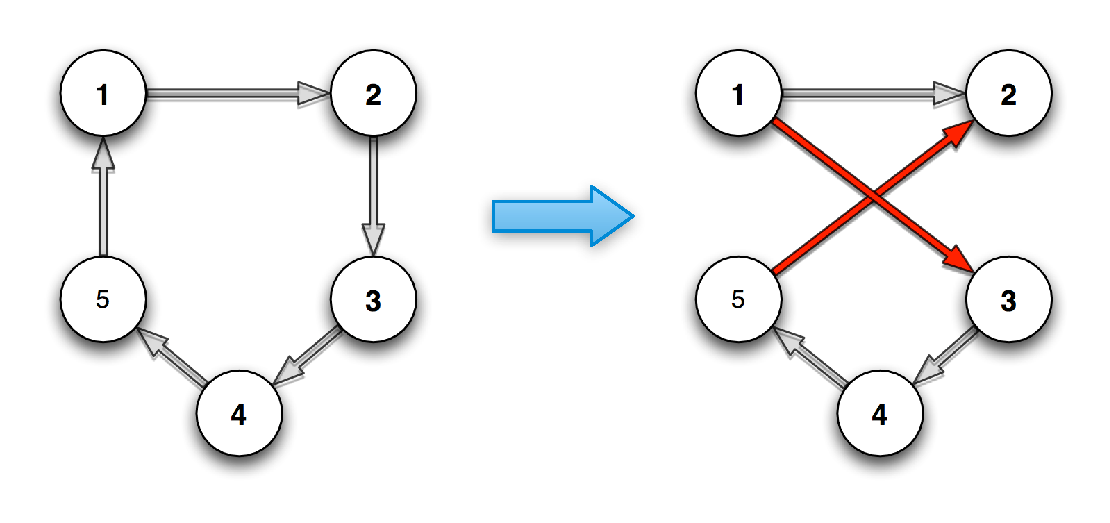
\includegraphics[width=0.90\linewidth]{rev_edge_graph.eps}
	\end{center}
	\caption{Exchanging edges}
	\label{exchange}
\end{figure}


Looking at the graph this way we it is clear that we can divide it into two disjoint sets with the exchanged edges being the interconnection between the two. Since each half in itself is correctly directed to create a new directed graph of the union of the disjoint sets only one of the two sets needs to be reversed. A local optimization we investigated was if we where able to determine or at least approximate the size of each set we could make reversing edges more efficient by choosing the smaller set. 

To calculate the size of any of the sets we must be able to determine its size for any node since the edges picked for exchange can be picked arbitrarily. This means the the only way to determine the size of the set is to traverse set linearly starting and stopping in any of the two nodes involved in the edge exchange. If we denote the size of a graph as $|N|$ and the size of the two disjoint sets as $|A|$ resp. $|B|$ we then know that $|B| = |N| - |A|$ this means that if we, while calculating the size for $A$, come to a point where $|A| > \frac{|N|}{2}$ we can conclude that $B$ is smaller and then reverse the edges of the set $B$. The problem with this approach is that if we while investigating the size of a set conclude that the \textit{other} set is smaller and reverse that set the result would be that we have visited $|N|$ nodes in total which is not desired. 

The argument above also shows that no other approximation is possible and we further believe that the use of additional data structures to keep track of set size for various nodes is not possible due the fact that edges can be exchange at random as shown above.

In our implementation we simply pick the set arbitrarily and reverse the edges of that set. Since the edges involved in the 2OPT exchange is picked at random and we pick one set out of two who's union forms the entire graph we state, without proof that the average size of the set picked will have have a size of $\frac{1}{2} \times |N|$.


\section{Repeated iterations}

As with any (likely) polynomial solution to this problem, we're going to get stuck in a local maxima. By using non-deterministic iteration order to either tour-construction algorithms or our locally optimizing algorithms, we should (and experimentally do) get stuck in different maximas. Repeating the tour-generation process will then generate more solutions. If we choose the best of more constructed tours, we're likely to get a better result on average. This was very successful for us, and we managed to score a few more points off of it simply by having a random starting point for the 2-opt step.

We'd recommend trying different initial tours as well, as greedy shown to be better in some cases where nearest neighbour didn't. This wasn't something that we had time to implement however, but it could prove valuable.

\begin{thebibliography}{9}

\bibitem{localopt}
	D. Johnson and L. McGeoch,
	\emph{The Traveling Salesman Problem: A Case Study in Local Optimization. in Local Search in Combinatorial Optimization}.
	E. H. L. Aarts and J. K. Lenstra (eds), John Wiley and Sons, Ltd., 1997, pp. 215-310. http://www2.research.att.com/~dsj/papers.html

\bibitem{kattis}
	Kattis
	\emph{Travelling Salesperson 2D}
	https://kth.kattis.scrool.se/problems/oldkattis:tsp

\bibitem{bound}
	D. S. Johnson, L. A. McGeoch, E. E. Rothberg
	\emph{Asymptotic Experimental Analysis for the Held-Karp Traveling Salesman Bound}
	Proceedings of the 7th Annual ACM-SIAM Symposium on Discrete Algorithms (1996), 341-350. http://public.research.att.com/~dsj/papers/HKsoda.pdf

\bibitem{lk}
	K. Helsgaun
	\emph{An Effective Implementation of the Lin-Kernighan Traveling Salesman Heuristic}
	Department of Computer Science, Roskilde University. \url{http://www.akira.ruc.dk/~keld/research/LKH/LKH-2.0/DOC/LKH_REPORT.pdf}
\end{thebibliography}

\bibitem{exact}
	Richard M. Karp
	\emph{Dynamic programming meets the principle of inclusion and exclusion}
	Computer Science Division, University of California. \url{http://dx.doi.org/10.1016%2F0167-6377%2882%2990044-X}
\end{document}

